\documentclass{presentation}

\title{3D Printing}
\subtitle{In the Chemistry Instrument Shop}
\author{Blaise Thompson}

\institute{University of Wisconsin--Madison}
\date{\today}

\begin{document}
\maketitle

\section{Introduction}

\begin{frame}{3D Printing}
  \begin{itemize}
    \item can be cheap
    \item slow (wall time)
    \item fast (human time)
  \end{itemize}
\end{frame}

\begin{frame}{Types of 3D Printing}
  \begin{itemize}
    \item stereolithography (SLA)
    \item selective laser sintering (SLS)
    \item fused deposition modeling (FDM)
  \end{itemize}
\end{frame}


\section{Stratasys}

\begin{frame}{Our Printer}
  UPrint SE Plus
  \begin{itemize}
    \item only one material: ABS
    \item soluble support (proprietary)
    \item build plates
    \item temperature controlled environment
    \item layer thickness 10 thousandths of an inch
    \item minimum wall thickness 36 thousandths of an inch
    \item build volume 8''x8''x6''
  \end{itemize}
\end{frame}

\begin{frame}{ABS}
  Acrylonitrile butadiene styrene
  \begin{itemize}
    \item glass transition 105 C
    \item poor chemical compatibility with organic solvents
    \item \$3 per cubic inch
  \end{itemize}
\end{frame}

\section{Design}

\begin{frame}{Design Tips}
  
\includegraphics[width=\textwidth]{./design-tips.jpg}
\end{frame}

\begin{frame}{Design Tips}
  \centering
  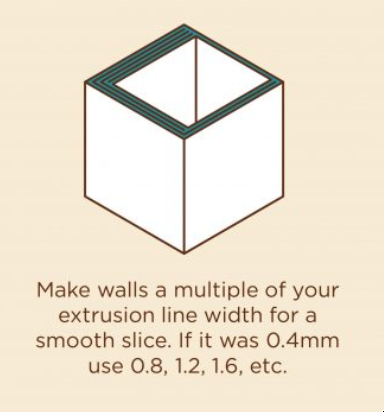
\includegraphics[width=\textwidth/2]{./multiple.jpg}
\end{frame}

\begin{frame}{Design Tips}
  \centering
  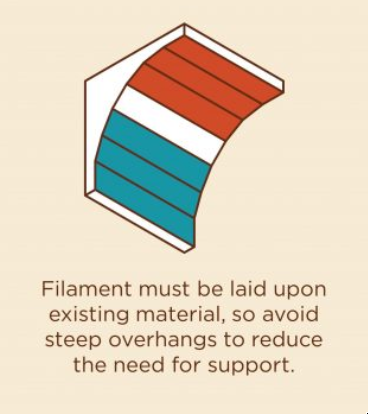
\includegraphics[width=\textwidth/2]{./overhang.jpg}
\end{frame}

\begin{frame}{Design Tips}
  \centering
  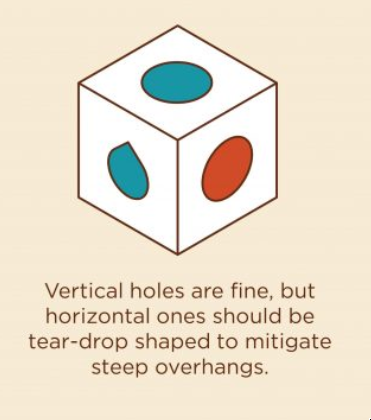
\includegraphics[width=\textwidth/2]{./holes.jpg}
\end{frame}

\begin{frame}{Design Tips}
  \centering
  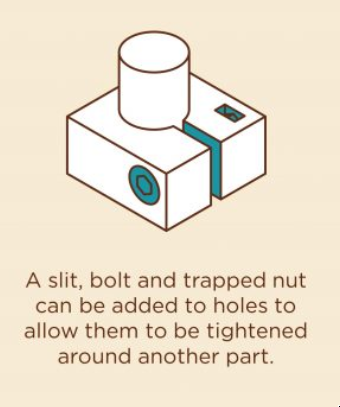
\includegraphics[width=\textwidth/2]{./trapped-nut.jpg}
\end{frame}

\begin{frame}{Design Tips}
  \centering
  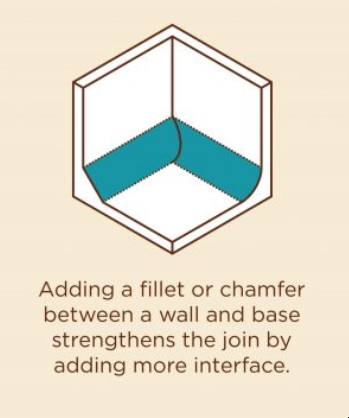
\includegraphics[width=\textwidth/2]{./chamfer.jpg}
\end{frame}

\begin{frame}{Design Tips}
  \centering
  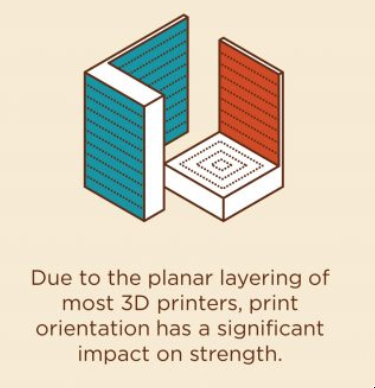
\includegraphics[width=\textwidth/2]{./strength.jpg}
\end{frame}

\begin{frame}{Design Tips}
  \centering
  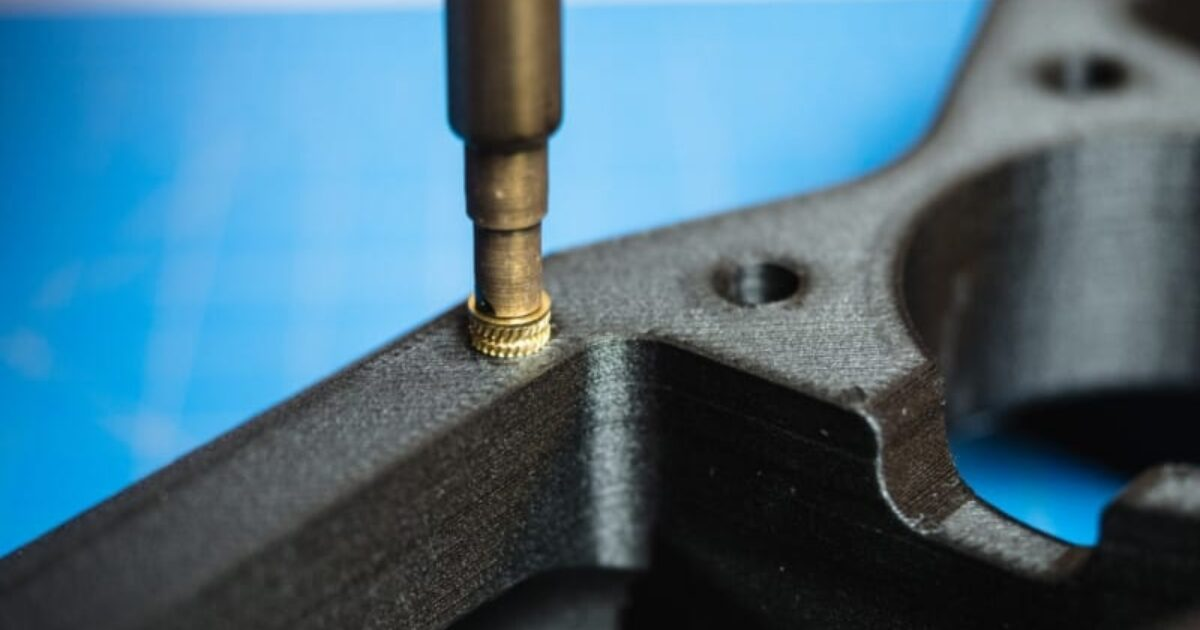
\includegraphics[width=\textwidth]{./heatset}
\end{frame}

\begin{frame}{Design Tips}
  \centering
  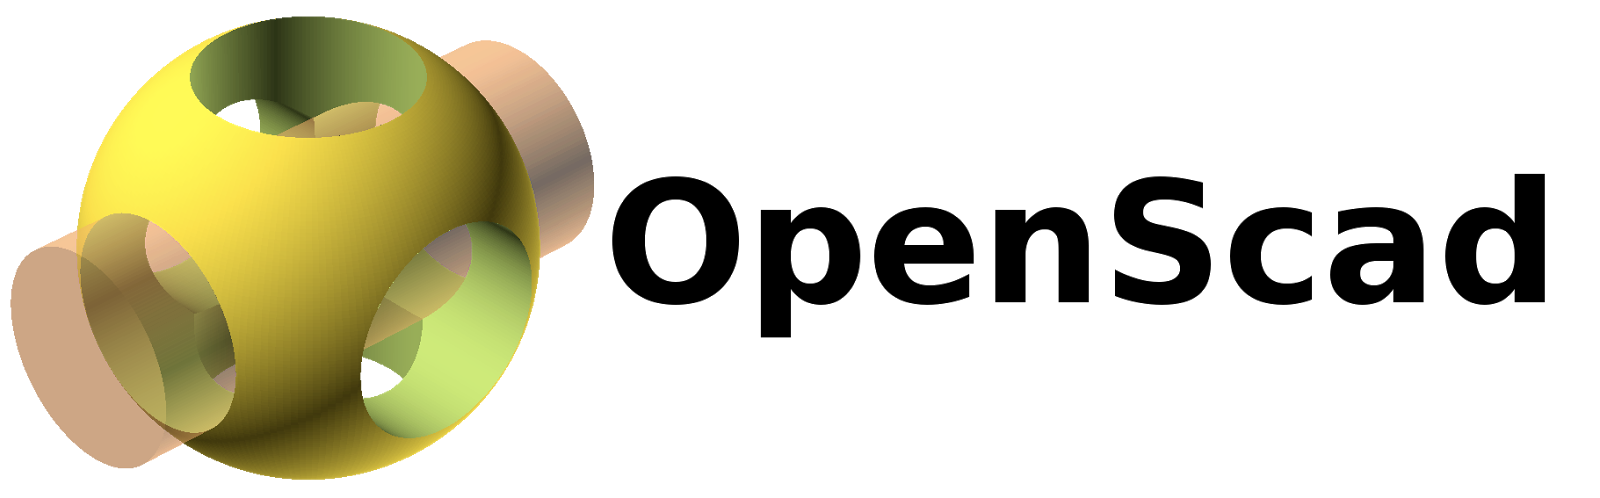
\includegraphics[width=\textwidth]{./OPENSCADLOGO.png}
\end{frame}

\section{Conclusion}

\begin{frame}{Conclusion}
  Thanks for your attention!
\end{frame}

\end{document}
